\documentclass{beamer}
\usepackage{beamerthemesplit}
\usepackage{booktabs}
\usepackage{graphicx}
\usepackage{transparent}
\usepackage{bbold}
\usepackage[italian]{babel}
\usepackage[utf8x]{inputenc}
\usepackage{listings}
\usepackage{tikz}
\usetikzlibrary{arrows}
\usepackage{amsmath,amsfonts,amssymb}
\usepackage{pgfplots}
\usepackage{scalefnt}
\usepackage{color}
\usepackage{xcolor}
\usepackage{multicol}
\usepackage{bm}

\title[mRMR]{mRMR - features selection method}
\institute{
\begin{small}
Corso di Laurea in Informatica Magistrale
\end{small}}
\author{\textbf{Simone Rutigliano}}
\date{\tiny{\today}}

\usebackgroundtemplate{
%    \transparent{0.12}{
     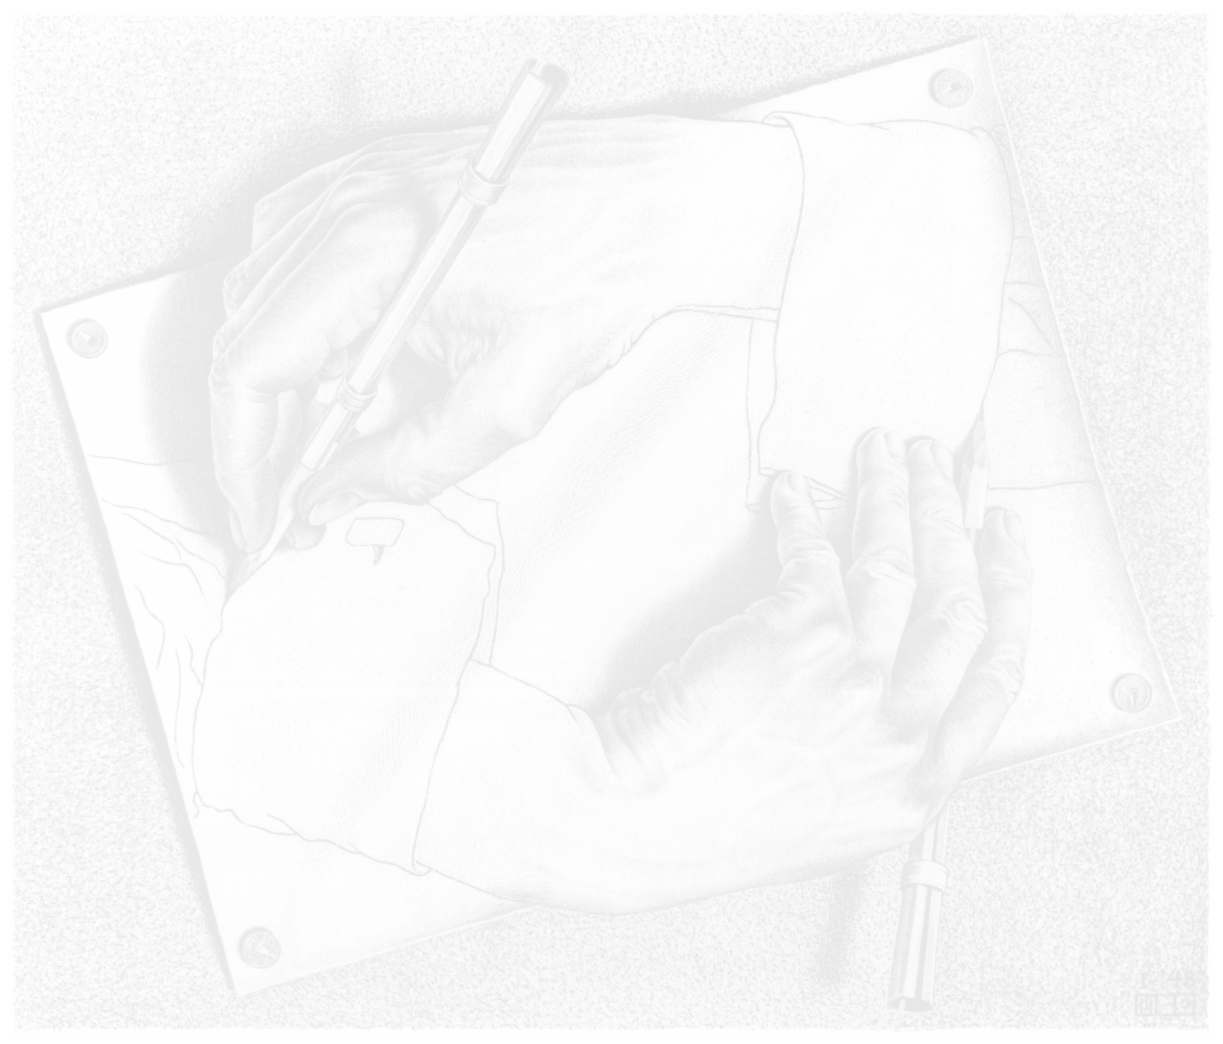
\includegraphics[width=\paperwidth, height=\paperheight]{./figure/theme/escher_hands_tr.png}
%    }
}

%\usetheme{Hannover}
\usetheme{Copenhagen}
\usecolortheme{seahorse}
\usecolortheme{rose}
%\usetheme{Frankfurt}
%\usecolortheme{beetle}

%\useoutertheme[subsection=false]{smoothbars}
%\useoutertheme[subsection=false]{smoothtree}
\useoutertheme{shadow}
\setbeamercovered{dynamic}

\pgfdeclareimage[height=1cm]{logo}{figure/theme/logo}
\logo{\pgfuseimage{logo}}

\begin{document}

%%%%%%%%%%%%%%%%%%%%%%%%%%%%%%%%%%%%%%%%%%%%%%%%%%%%%

\begin{frame}
\maketitle
\end{frame}

%%%%%%%%%%%%%%%%%%%%%%%%%%%%%%%%%%%%%%%%%%%%%%%%%%%%%

\begin{frame}
\frametitle{Outline}
	\begin{multicols}{2}
		\tableofcontents
	\end{multicols}
\end{frame}

%%%%%%%%%%%%%%%%%%%%%%%%%%%%%%%%%%%%%%%%%%%%%%%%%%%%%
\section{Mutual Information}
\subsection{Definizione}
\begin{frame}
	\frametitle{Definizione}
		\nocite{Ding:2003:MRF:937976.938050}
		\nocite{Peng05featureselection}
Date due variabili casuali \emph{X} e \emph{Y} con distribuzione di probabilità congiunta $p(x, y)$, la mutua
informazione è definita come \\~$$I(X; Y ) = H(X) − H(X|Y ) = H(Y ) − H(Y |X)$$\\~\\
La mutua informazione rappresenta i bit di informazione che una delle variabili fornisce circa l'altra
\begin{figure}[htb]
	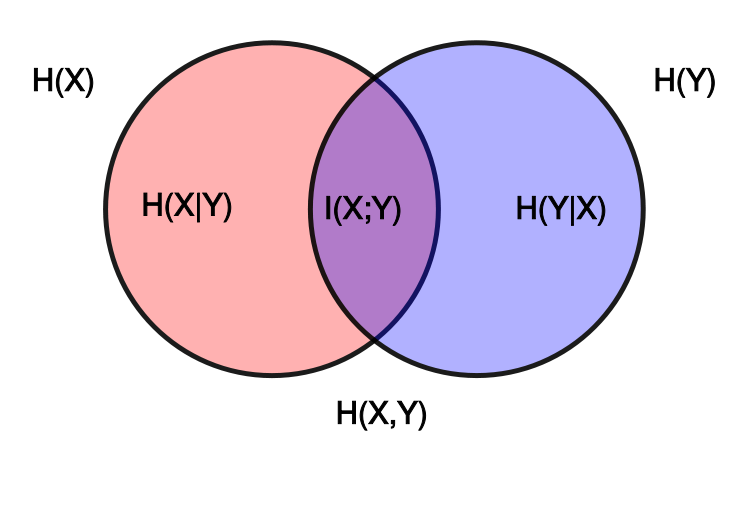
\includegraphics[width=0.50\textwidth]{figure/mutual.png}
\end{figure}
\end{frame}
\begin{frame}
	\frametitle{Considerazioni}
	\begin{itemize}
		\item $I(X;Y)=0 \Rightarrow$ \emph{X} e \emph{Y} sono variabili indipendenti
		\item $\pmb{I(X;Y)} = H(X)-H(X|Y)=H(Y)-H(Y|X)= \pmb{I(Y;X)}$
		\item $I(X;X)=H(X)$
	\end{itemize}
\end{frame}
\begin{frame}
	\frametitle{Esempio}
	Lanciamo 10 monete:
	\begin{itemize}
		\item \emph{X} rappresenta i valori delle prime 7 monete
		\item Y quelli delle ultime 5
	\end{itemize}
	Avremo che:
	\begin{columns}
		\begin{column}{0.5\textwidth}
			\begin{itemize}
				\item $H(X) = 7$
				\item $H(Y ) = 5$\newline
			\end{itemize}
		\end{column}
		\begin{column}{0.5\textwidth}
			\begin{itemize}
				\item $H(X|Y ) = 5$
				\item $H(Y|X) = 3$\newline
			\end{itemize}
		\end{column}
	\end{columns}
	La mutua informazione sarà quindi pari a
$$I(X; Y ) = I(Y ; X) = 2 $$
\end{frame}
\subsection{Formule}
\begin{frame}
	\frametitle{Discrete}
	Definite due variabili casuali discrete \emph{X} e \emph{Y}
	$$ I (x;y) = \sum\limits_{y \in Y} \sum\limits_{x \in X} p(x,y)\log \frac{p(x,y)}{p(x)p(y)}$$
	dove
	\begin{itemize}
		\item $p(x,y)$ è la funzione di distribuzione di probabilità congiunta di \emph{X} e \emph{Y}
		\item $p(x)$ e $p(y)$ sono le funzioni di distribuzione di probabilità marginale di X e Y
	\end{itemize}
\end{frame}
\begin{frame}
	\frametitle{Continuous}
	$$ I (x;y) = \int_Y \int_X p(x,y)\log \frac{p(x,y)}{p(x)p(y)} \mathrm{d}x \mathrm{d}y$$
	dove
	\begin{itemize}
		\item $p(x,y)$ è la funzione di densità di probabilità congiunta di \emph{X} e \emph{Y}
		\item $p(x)$ e $p(y)$ sono le funzioni di densità di probabilità marginale di X e Y
	\end{itemize}
\end{frame}
\subsection{Problematiche}
\begin{frame}
	\frametitle{Problematiche}
	In caso di variabili continue, difficoltà nella computazione degli integrali nello spazio continuo su un numero limitato di campioni\newline\newline
	\textbf{Soluzione}\newline\newline
	Incorporare la discretizzazione dei dati nella fase di preprocessing
\end{frame}

%%%%%%%%%%%%%%%%%%%%%%%%%%%%%%%%%%%%%%%%%%%%%%%%%%%%%

\section{Max Dependency}
\subsection{Definizione}
\begin{frame}
	\frametitle{Max Dependency}
	In terms of mutual information, the purpose of feature selection is to find a feature set S with m features fx i g, which jointly have the largest dependency on the target class c.
	$$ \max Dep(S,c), Dep = I(\{x_i,i=1,\dots,m \};c )$$
\end{frame}


\subsection{Formula}
\begin{frame}
	\frametitle{Max Dependency}

	

\end{frame}
\subsection{Problemi}
\begin{frame}
	
\end{frame}

%%%%%%%%%%%%%%%%%%%%%%%%%%%%%%%%%%%%%%%%%%%%%%%%%%%%%

\section{Max Relevance}
\subsection{Definizione}
\subsection{Formule}
\begin{frame}
	\frametitle{Per variabili discrete}
	$$\max D(S,c), D= \frac{1}{|S|} \sum\limits_{x_i \in S} I (x_i;c)$$
\end{frame}
\begin{frame}
	\frametitle{Per variabili continue}
\end{frame}
\subsection{Problematiche}
\begin{frame}
	\frametitle{ridondanza}
	si incorre nel problema della ridondanza
\end{frame}

%%%%%%%%%%%%%%%%%%%%%%%%%%%%%%%%%%%%%%%%%%%%%%%%%%%%%
\section{Min Redundancy}
\subsection{Definizione}
\begin{frame}
	contenuto...
\end{frame}
\subsection{Formule}
\begin{frame}
	\frametitle{Per variabili discrete}
	$$\min R(S), D= \frac{1}{|S|^2} \sum\limits_{x_i,x_j \in S} I (x_i;x_j)$$
\end{frame}
\begin{frame}
	\frametitle{Per variabili continue}
\end{frame}

%%%%%%%%%%%%%%%%%%%%%%%%%%%%%%%%%%%%%%%%%%%%%%%%%%%%%

\section{mRMR}
\subsection{Definizione}
\begin{frame}
	\frametitle{Def}
\end{frame}

\subsection{Formule}
\begin{frame}
	\frametitle{Discrete - MID}
	$$\max \Phi(D,R), \Phi = D - R$$
	dove $D=I(i,h)$ e $R=\frac{1}{|S|}\sum\limits_{j \in S}I(i,j)$
\end{frame}

\begin{frame}
	\frametitle{Discrete - MIQ}
	$$\max \Phi(D,R), \Phi = \frac{D}{R}$$
\end{frame}
\begin{frame}
	\frametitle{Continuous}
	$$ F(g_i,h) = \frac{\frac{\sum\limits_{K}{n_k(\bar{g_k}-\bar{g})}}{K-1}}{\sigma^2}$$
	dove: $\sigma^2=\frac{ \sum\limits_{k}{(n_k-1)\sigma^2_k}}{n-K}$
\end{frame}
\begin{frame}
	\frametitle{Continuous - FCD}
\end{frame}

\begin{frame}
	\frametitle{Continuous - FCQ}
\end{frame}

\subsection{Benefici}
\begin{frame}
	\frametitle{Benefici}
\end{frame}
%%%%%%%%%%%%%%%%%%%%%%%%%%%%%%%%%%%%%%%%%%%%%%%%%%%%%

\begin{frame}{Bibliography}
	\frametitle{References}
	\bibliographystyle{alpha}
	\bibliography{mybib}
\end{frame}
\end{document}
